% Options for packages loaded elsewhere
\PassOptionsToPackage{unicode}{hyperref}
\PassOptionsToPackage{hyphens}{url}
%
\documentclass[
]{article}
\title{OPINIÃO PÚBLICA DOS RELIGIOSOS ACERCA DA TOLERÂNCIA POLÍTICA AOS
HOMOSSEXUAIS NA AMÉRICA LATINA}
\author{Discente: Naiara Sandi de Almeida Alcantara //Orientador:
Ednaldo Aparecido Ribeiro}
\date{02, agosto 2022}

\usepackage{amsmath,amssymb}
\usepackage{lmodern}
\usepackage{iftex}
\ifPDFTeX
  \usepackage[T1]{fontenc}
  \usepackage[utf8]{inputenc}
  \usepackage{textcomp} % provide euro and other symbols
\else % if luatex or xetex
  \usepackage{unicode-math}
  \defaultfontfeatures{Scale=MatchLowercase}
  \defaultfontfeatures[\rmfamily]{Ligatures=TeX,Scale=1}
\fi
% Use upquote if available, for straight quotes in verbatim environments
\IfFileExists{upquote.sty}{\usepackage{upquote}}{}
\IfFileExists{microtype.sty}{% use microtype if available
  \usepackage[]{microtype}
  \UseMicrotypeSet[protrusion]{basicmath} % disable protrusion for tt fonts
}{}
\makeatletter
\@ifundefined{KOMAClassName}{% if non-KOMA class
  \IfFileExists{parskip.sty}{%
    \usepackage{parskip}
  }{% else
    \setlength{\parindent}{0pt}
    \setlength{\parskip}{6pt plus 2pt minus 1pt}}
}{% if KOMA class
  \KOMAoptions{parskip=half}}
\makeatother
\usepackage{xcolor}
\IfFileExists{xurl.sty}{\usepackage{xurl}}{} % add URL line breaks if available
\IfFileExists{bookmark.sty}{\usepackage{bookmark}}{\usepackage{hyperref}}
\hypersetup{
  pdftitle={OPINIÃO PÚBLICA DOS RELIGIOSOS ACERCA DA TOLERÂNCIA POLÍTICA AOS HOMOSSEXUAIS NA AMÉRICA LATINA},
  pdfauthor={Discente: Naiara Sandi de Almeida Alcantara //Orientador: Ednaldo Aparecido Ribeiro},
  hidelinks,
  pdfcreator={LaTeX via pandoc}}
\urlstyle{same} % disable monospaced font for URLs
\usepackage[margin=1in]{geometry}
\usepackage{graphicx}
\makeatletter
\def\maxwidth{\ifdim\Gin@nat@width>\linewidth\linewidth\else\Gin@nat@width\fi}
\def\maxheight{\ifdim\Gin@nat@height>\textheight\textheight\else\Gin@nat@height\fi}
\makeatother
% Scale images if necessary, so that they will not overflow the page
% margins by default, and it is still possible to overwrite the defaults
% using explicit options in \includegraphics[width, height, ...]{}
\setkeys{Gin}{width=\maxwidth,height=\maxheight,keepaspectratio}
% Set default figure placement to htbp
\makeatletter
\def\fps@figure{htbp}
\makeatother
\setlength{\emergencystretch}{3em} % prevent overfull lines
\providecommand{\tightlist}{%
  \setlength{\itemsep}{0pt}\setlength{\parskip}{0pt}}
\setcounter{secnumdepth}{-\maxdimen} % remove section numbering
\ifLuaTeX
  \usepackage{selnolig}  % disable illegal ligatures
\fi

\begin{document}
\maketitle

{
\setcounter{tocdepth}{3}
\tableofcontents
}
\hypertarget{introduuxe7uxe3o}{%
\section{Introdução}\label{introduuxe7uxe3o}}

\hypertarget{objetivo}{%
\subsection{Objetivo:}\label{objetivo}}

\begin{enumerate}
\def\labelenumi{\arabic{enumi}.}
\tightlist
\item
  Constatar a relação entre religião e tolerância política em países da
  América Latina e identificar quais aspectos religiosos são mais
  proeminentes no ato de tolerar
\end{enumerate}

``Utilizamos medidas que analisam três aspectos religiosos, em
conformidade com a tríade: 1) comportamentos, 2) pertencimento, 3) e
crenças (no inglês, The Three Bs: behavior, belonging e beliefs) (LEEGE;
KELLSTEDT; WALD, 1996).'' \vspace{5truemm}

\hypertarget{material-empuxedrico}{%
\subsection{Material Empírico:}\label{material-empuxedrico}}

Surveys fornecidos pelo Latin American Public Opinion Project (LAPOP)
Período analisado: 2014, 2016/2017 e 2018/2019

\hypertarget{pauxedses}{%
\subsection{Países:}\label{pauxedses}}

\textbf{Brasil, Uruguai, El Salvador e Guatemala} (i)

\begin{center}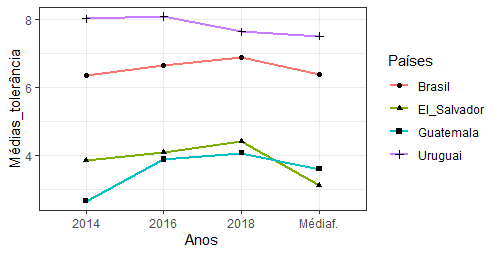
\includegraphics[width=0.8\linewidth]{Rplot} \end{center}

\hypertarget{hipuxf3tese}{%
\subsection{Hipótese:}\label{hipuxf3tese}}

H1 - Países com os menores índices de tolerância possuem indivíduos
ativos religiosamente, que atribuem maior importância a religião e são
filiados a denominações religiosas mais conservadoras. Acredita-se que
as três variáveis citadas sejam fortes preditoras da diminuição da
tolerância política em dois dos países analisados, pois possuem as
menores médias simples de tolerância.

``Quadro 1 - Síntese dos direitos dos homossexuais nos países que
comporão a tese (ii)''

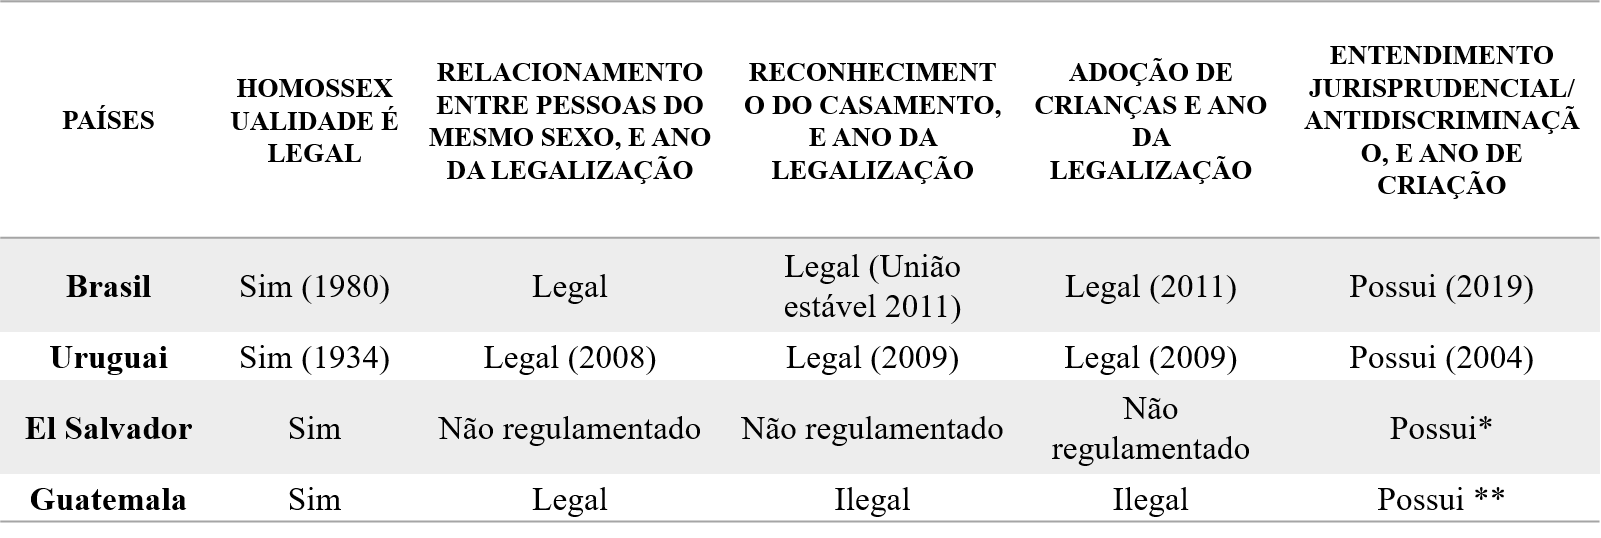
\includegraphics{//cloud/project/Imagens2/Imagem4.png} *Algumas leis
contrárias à discriminação ** Antidiscriminação na Lei da Infância e da
Juventude desde 1997 Fonte: Autora, 2021, a partir da legislação dos
países.

\vspace{5truemm}

\hypertarget{dados-objetivos-e-metodologia}{%
\section{Dados, objetivos e
Metodologia}\label{dados-objetivos-e-metodologia}}

\hypertarget{metodologia-quantitativa}{%
\subsection{Metodologia: Quantitativa}\label{metodologia-quantitativa}}

\hypertarget{dados}{%
\subsection{Dados:}\label{dados}}

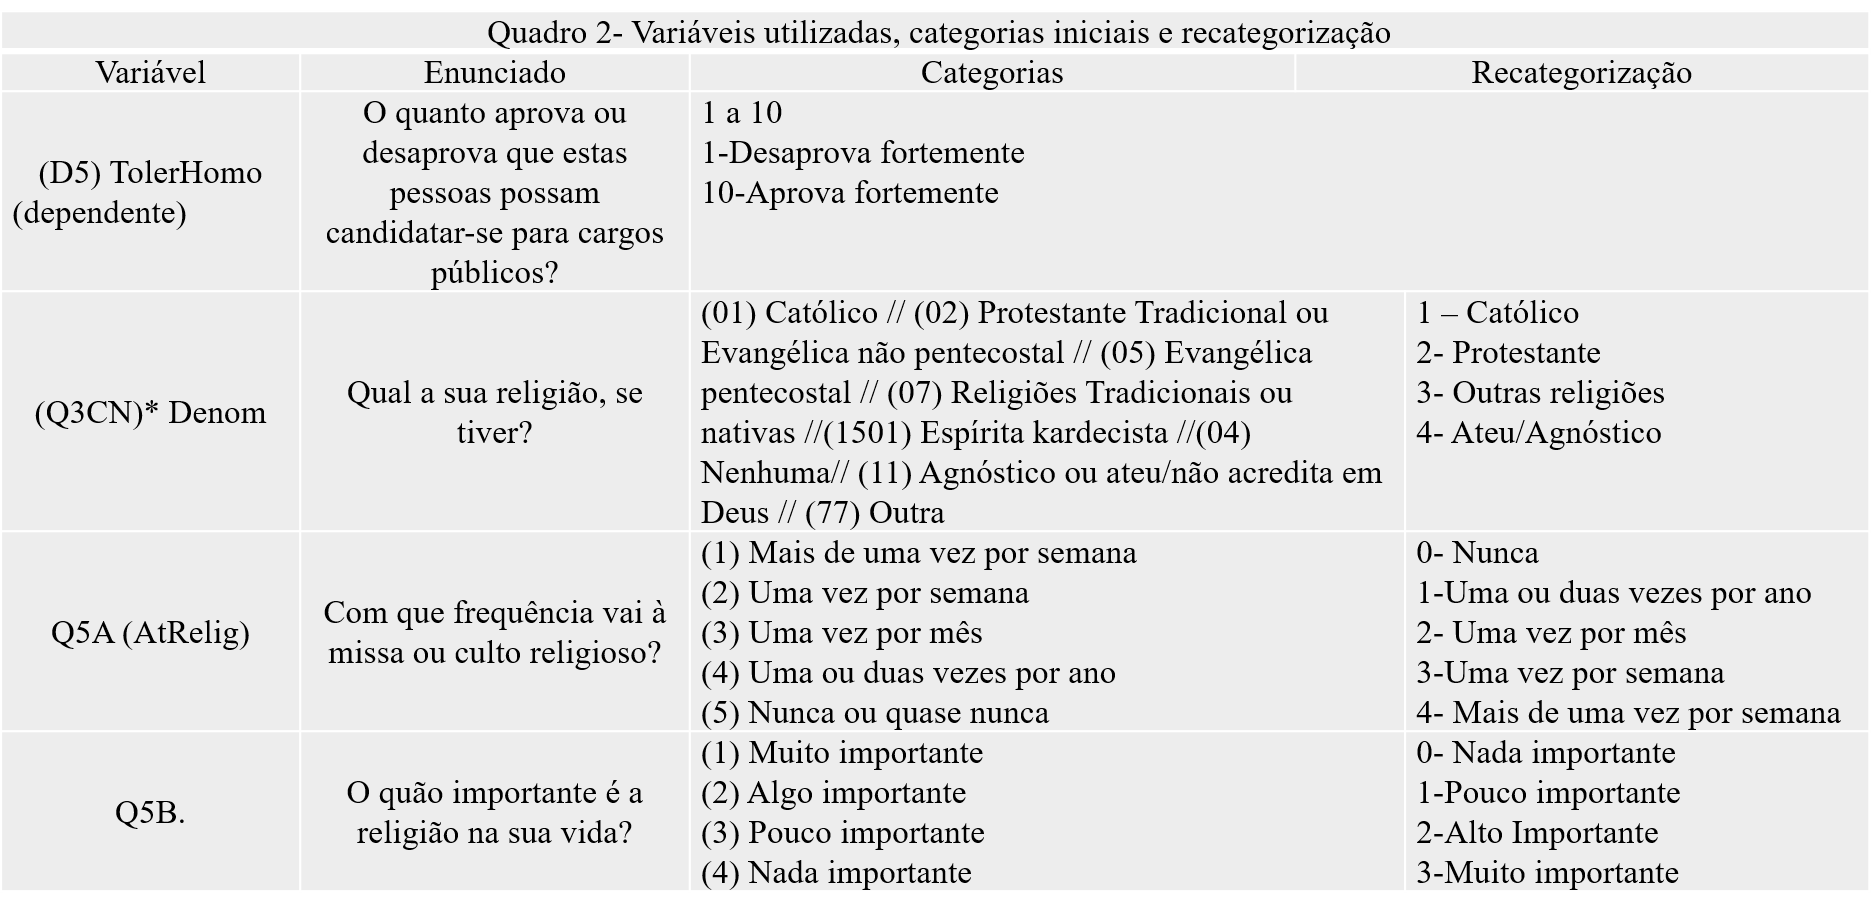
\includegraphics{//cloud/project/Imagens2/tabela5.png}

*Obs.: As categorias originais dessa variável mudam a depender do ano de
aplicação ou do país, mas todos possuem as denominações: católica,
protestante, outras denominações e ateu/agnóstico, por isso foi possível
realizar a mesma recategorização idêntica para todos os casos. Fonte:
Autora, a partir do dicionário de códigos do LAPOP Brazil, 2019

\vspace{5truemm}

\hypertarget{descritivas}{%
\subsection{Descritivas:}\label{descritivas}}

Gráfico 1 -- Projeções gráficas do total de observações por ano em cada
país analisado e da frequência de cada denominação religiosa

\begin{center}\includegraphics{Apresentação-Naiara_files/figure-latex/unnamed-chunk-4-1} \end{center}

\vspace{5truemm}

\hypertarget{resultados}{%
\section{Resultados}\label{resultados}}

Tabela 1- Influência da religião sobre a tolerância política em relação
aos homossexuais em quatro países da América Latina 2014

\begin{center}
\includegraphics[width=0.8\linewidth]{tabela1} \end{center}

Fonte: Autora, a partir LAPOP

Tabela 2- Influência da religião sobre a tolerância política em relação
aos homossexuais em quatro países da América Latina 2016/2017

\begin{center}
\includegraphics[width=0.8\linewidth]{tabela2} \end{center}

Fonte: Autora, a partir LAPOP

Tabela 3- Influência da religião sobre a tolerância política em relação
aos homossexuais em quatro países da América Latina 2018/2019

\begin{center}
\includegraphics[width=0.8\linewidth]{tabela3} \end{center}

Fonte: Autora, a partir LAPOP

\vspace{5truemm}

\hypertarget{considerauxe7uxf5es-finais}{%
\section{Considerações finais}\label{considerauxe7uxf5es-finais}}

Apesar da hipótese inicial ter sido apenas parcialmente confirmada,
acredita-se que a principal contribuição do artigo é demonstrar que em
pelo menos um aspecto religioso, a filiação denominacional (belonging),
há evidências de forte influência na diminuição da tolerância política
aos homossexuais. Muito embora, não seja possível afirmar que a religião
seja a causa da intolerância, já que os testes não apresentam resultados
referentes a causalidade, pode-se inferir que existem relações e
correlações, e conforme aumenta a frequência religiosa, bem como, a
filiação a denominação protestente, aumenta também a tendencia de
atitudes de intolerância aos gays e lésbicas.

\end{document}
